\chapter{Analyse}\label{cha:analysis}

In dit hoofdstuk passen we het model zodanig aan dat het aansluit op de context van de kraslotenactie. We verfijnen eerst het model door een vergelijking op te stellen van de verwachtingswaarde en de variantie van onze totale uitgaven, bestaande uit verschillende nog te bepalen parameters. Wij proberen een ``juiste'' invulling te geven aan deze parameters door het gedrag te bestuderen van de variantie, wanneer we met deze parameters spelen. Verder kijken we naar de invloed van parameter $p$ en we sluiten het hoofdstuk af met een zekerheidsanalyse.

\section{Verwachte uitgave}

We stellen onze vergelijkingen op vanuit het perspectief van het aantal identieke symbolen dat is opengekrast. Elk type lot ($\alpha$ t/m $\zeta$ zoals beschreven in hoofdstuk 2) heeft een vast aantal bedragen dat gewonnen kan worden (bijv. met een lot van het type $\gamma$ kun je \euro25 en \euro10 winnen). We kunnen dan met behulp van de hypergeometrische verdeling $V$ bepalen welk bedrag is gewonnen bij de combinatie van gelijke symbolen. Daarnaast gebruiken we de binomiale verdeling $X$ om het aantal klachteloze vrije dagen erbij te betrekken, waarbij we conditioneel te werk gaan voor $x=0,\ldots,6$.

We moeten dus een functie introduceren die aan een aantal identieke symbolen dat is opengekrast een prijs toekent. We maken hierbij de opmerking dat we bij 6 opengekraste gelijke symbolen geen standaard prijs kunnen noteren. Hier gaan we later afzonderlijk op in en dus noteren we voor nu een gewonnen bedrag van \euro0. Ditzelfde geldt voor loten van het type $\zeta$ waar bonusstapelpunten mee verdiend kunnen worden. Wij defini\"eren de waardefunctie (``prijsfunctie'') $g$ als volgt:
\begin{equation}
  g(v|x,\sigma)_{p} =
  \begin{cases}
     0 & v = 6\\
    50 & v = 5\\
    25 & v = 4\\
    10 & v = 3\\
    0 & anders
  \end{cases}
\end{equation}

We introduceren nu de nieuwe random variabele $g(V|X,\Sigma)_{p}$. Deze staat voor de door de bezorger gewonnen prijs voor een lot waarop een combinatie van $v$ identieke plaatjes is opengekrast. Hierbij geeft $X$ weer hoeveel klachteloze dagen er in week zijn en $\Sigma$ zegt over welk type lot we het hebben. Tot slot geeft $p$ de kans weer dat er sprake is van een klachteloze vrije dag. Deze kans is variabel tussen de 0,75 en 0,90. We willen voor één lot van het type $\sigma$ graag bepalen wat de verwachte winst is voor de bezorger, ofwel het verwachte ``verlies'' dat wij als organisatie lijden. Gebruikmakende van de conditionele verwachtingswaarde krijgen we dat:

\begin{equation}
  \mathbb{E}[g(V|X,\Sigma)_{p}] = \sum_{x=0}^{6} \Bigg[ \sum_{v=0}^{\sigma} g(v|x,\sigma)_{p} * f_{V|X,\Sigma}(v|x,\sigma) \Bigg] \binom{6}{x} p^{x}(1-p)^{6-x}
\end{equation}

Nu we de verwachtingswaarde van één lot van het type $\sigma$ kunnen bepalen, zijn we natuurlijk ook in staat om de verwachtingswaarde van $x$ loten van het type $\sigma$ te bepalen. We introduceren nu een extreem belangrijke som van random variabelen.

\begin{equation}
\alpha g(V|X,6)_{p} + \beta(V|X,5)_{p} + \gamma g(V|X,4)_{p} + \delta g(V|X,3)_{p} + \zeta g(V|X,0)_{p}
\end{equation}

Deze som van random variabelen geeft het totale prijzengeld (ofwel onze uitgaven) weer dat met de krasloten gewonnen wordt gedurende precies één week. Het mag echter duidelijk zijn dat deze random variabele nog niet compleet is. Immers zit het geld dat gewonnen wordt in de grote pot van krasloten met 6 identieke symbolen en met de bonusstapelpunten nog niet hierin verwerkt. Bovendien mogen we $\zeta g(V|X,0)_{p}$ weglaten, omdat deze altijd een waarde van 0 aanneemt (dit type lot valt altijd onder de categorie ``anders'' in (3.1)).\\

We bespreken nu eerst hoe we het winnen van de bonusstapelpunten verwerken. We zetten uiteraard de mogelijke gewonnen aantallen stapelpunten om in euro's (respectievelijk \euro2,50; \euro5; \euro7,50; \euro0). We moeten een nieuwe randomvariabele introduceren, namelijk $h(V|X,0)_{p}$. Deze geeft de gewonnen prijs weer van een lot van het type $\zeta$. Verder is de functie $h(v|x,0)_{p}$ als volgt gedefinieerd:

\begin{equation}
  h(v|x,0)_{p} =
  \begin{cases}
    2,50 & x = 6 \mbox{ en ``subtype lot''}= a \\
    5 & x = 6 \mbox{ en ``subtype lot''}= b \\
    7,50 & x = 6 \mbox{ en ``subtype lot''}= c \\
    0 & x = 6 \mbox{ en ``subtype lot''}= d \\
    0 & \mbox{anders}
  \end{cases}
\end{equation}

Indien een lot (van het type $\zeta$) voldoet aan de eisen om stapelpunten te verdienen, kent $h(V|X,0)_{p}$ een aantal van $v$ opengekraste identieke symbolen, gegeven $x$ klachteloze vrije dagen om in een prijs van ofwel \euro2,50, \euro5 of \euro7,50. Merk op dat voor loten van het subtype $d$ de gewonnen prijs altijd gelijk is aan \euro0 en zodoende zal deze parameter niet meer optreden in de resterende vergelijkingen.

Het bepalen van $\mathbb{E}[h(V|X,0)_{p}]$ gaat op dezelfde manier als in (3.2), waarbij we functie g vervangen door functie h. Echter kunnen we deze dubbele sommering hevig versimpelen. Verdeling V is hier namelijk helemaal niet relevant (omdat we nu niet werken met combinaties van opengekraste identieke symbolen) en wat betreft verdeling X, deze geeft alleen een toevoeging aan de verwachtingswaarde wanneer alle zes de vakjes zijn opengekrast, ofwel wanneer $x=6$. Daarom mogen we zeggen dat:

\begin{equation}
\mathbb{E}[h(V|X,0)_{p}] = h(v|x,0)_{p}*f_{X}(6)
\end{equation}

We kunnen de som van random variabelen uit (3.3) nu dus aanvullen. Tevens korten we deze vanaf nu af tot $Z_{p}$, waarbij $Z_{p}$ dus staat voor de totale uitgaven (minus de gegarandeerde prijzenpot van \euro6000) gedurende precies één week. Deze luidt:

\begin{equation}
\begin{aligned}
Z_{p} = \alpha g(V|X,6)_{p} + \beta g(V|X,5)_{p} + \gamma g(V|X,4)_{p} + \delta g(V|X,3)_{p}  \\ 
+ a*h(V|X,0)_{0,p} +b*h(V|X,0)_{p} +c*h(V|X,0)_{p}
\end{aligned}
\end{equation}

De lineariteit van de verwachtingswaarde geeft ons dan:

\begin{equation}
\begin{aligned}
	\mathbb{E}\left[Z_{p} \right] &=
    \alpha\mathbb{E}[g(V|X,6)_{p}] + \beta\mathbb{E}[g(V|X,5)]_{p} \\
    &\qquad{}+ \gamma\mathbb{E}[g(V|X,4)]_{p} + \delta\mathbb{E}[g(V|X,3)]_{p}  \\
    &\qquad{}+ a[2,50f_{X}(6)_{p}] + b[5f_{X}(6)_{p}] + c[7,50f_{X}(6)_{p}]
\end{aligned}
\end{equation}

Zoals in hoofdstuk 2 behandeld is, gaan we ervan uit dat de 12 hoofdprijzen sowieso gewonnen worden. Daarom mogen we een standaard verlies van $4*250 + 4*500 + 4*750 = 6000$ toevoegen aan de uiteindelijke vergelijking. Om deze uiteindelijke vergelijking op te stellen hoeven we enkel 14 maal vergelijking (3.7) te sommeren voor 14 waarden waarden van $p$. Hierbij tellen we de gegarandeerde \euro6000 op en dit geeft ons de totale verwachtingswaarde van onze totaaluitgaven. We definiëren eerst T als zijnde de random variabele die staat voor de totaaluitgaven. Er geldt:

\begin{equation}
T = \sum_{i=1}^{14} Z_{p_{i}} + 6000.
\end{equation}

Met behulp van de lineariteit van de verwachtingswaarde kunnen we nu de gefinaliseerde vergelijking voor de verwachtingswaarde opstellen. Deze luidt:

\begin{equation}
\begin{aligned}
\mathbb{E}[T] &=& \mathbb{E}\left[\sum_{i=1}^{14} Z_{p_{i}} + 6000\right]\\
  &=& \mathbb{E}\left[\sum_{i=1}^{14} Z_{p_{i}} \right] + 6000\\
  &=&  \sum_{i=1}^{14} \left( \mathbb{E}[Z_{p_{i}}] \right) + 6000
\end{aligned}
\end{equation}

Merk op dat we nu niet meer werken met een algemene parameter $p$, maar met een variabele $p_{i}$. Deze geeft de kans weer op een klachteloze vrije dag gedurende de i'de week van de krasactie.

\begin{comment} -----------------------
Hier zit echter nog niet alles in verwerkt. Allereerst is het logisch dat het verwachte verlies voor loten van het type $\zeta$ gelijk is aan 0. (Daar valt immers niets conventioneels mee te winnen). We voegen nu de speciale prijzen toe aan deze vergelijking. Zoals in hoofdstuk 1 behandeld is, gaan we ervan uit dat de 12 hoofdprijzen sowieso gewonnen worden. Daarom mogen we nu vrij een standaard verlies van $4*250 + 4*500 + 4*750 = 6000$ toevoegen aan de uiteindelijke vergelijking. Omdat we nu per week kijken, laten we deze voor nu even buiten beschouwing. Verder zijn er ook bonusstapelpunten te verdienen voor mensen die een lot van het type $\sigma=0$ hebben ontvangen en die tevens een klachtenloze vrije week hebben gehad. We zetten hier natuurlijk de hoeveelheid stapelpunten om in de hoeveelheid geld die gewonnen kan worden (2,50; 5; 7,50). We zeggen dat er een totaal van $a$ loten zijn die een prijs van 2,50 weggeven, een totaal van $b$ loten die een prijs van 5 weggeven en een totaal van $c$ loten die een prijs van 7,50 weggeven. Omdat deze prijzen alleen weggegeven worden bij loten van het type $\zeta$ hoeven we hier geen rekening te houden met de andere typen loten. Daarom mogen we zeggen dat:

\begin{equation}
  a+b+c=\zeta
\end{equation}

De gefinaliseerde vergelijking luidt nu:

\begin{multline}
    \alpha\mathbb{E}[g(V)]_{6,p} + \beta\mathbb{E}[g(V)]_{5,p} + \gamma\mathbb{E}[g(V)]_{4,p} + \delta\mathbb{E}[g(V)]_{3,p}\\
        + a2,50f_{X}(6)_{p} + b5f_{X}(6)_{p} + c7,50f_{X}(6)_{p} = \mbox{ verwachte verlies in één week}
\end{multline}

De reden dat we naar het verwachte verlies per week kijken, is omdat we dan de kans op een klachtenloze vrije dag $p$ per week kunnen veranderen. Dit betekent dat we vegelijking (8) 14 keer moeten sommeren om het uiteindelijke verwachte verlies te bepalen. We korten vergelijking (3.5) voor het gemak even af als $\mathbb{E}_{p_{i}}$, waarbij $p_{i}$ de kans is op een klachteloze dag op een dag in de i'de week. Nu kunnen we een vergelijking opstellen voor de volledige uitgaven over 14 weken:

\begin{equation}
  \sum_{i=1}^{14} \left( \mathbb{E}_{p_{i}} \right) + 6000\\= \mbox{ totale verwachte verlies over 14 weken}
\end{equation}

Dit is dus de vergelijking die aangeeft hoeveel het verwachte verlies is dat wij in totaal zullen lijden. De opdrachtgever wenst dat dit verlies gelijk is aan 12.300. Aan ons is dus nu de taak een optimale verdeling te vinden voor $\alpha$, $\beta$, $\gamma$, $\delta$, $\zeta$, $a$, $b$ en $c$ zodanig dat vergelijking (9) gelijk is aan 12.300 en zodanig dat de kans dat deze sterk afwijkt zo klein mogelijk is. 
\end{comment} -------------------------

\section{Variantie}

In de vorige paragraaf hebben we een vergelijking opgesteld voor de verwachtingswaarde van de uitgaven over 14 weken. We zijn eigenlijk meer geïnteresseerd in de spreiding die aanwezig is, omdat we de opdrachtgever een bepaalde garantie willen bieden dat de uitgaven niet extreem veel zullen afwijken van de verwachtingswaarde. Dit kunnen we onderzoeken door naar de variantie te kijken.\\

Eerst bepalen we de variantie van de afzonderlijke random variabelen. Deze zullen we dadelijk nodig hebben als we de totale variantie willen bepalen. Er geldt per definitie dat:

\begin{eqnarray*}
  Var(g(V|X,\Sigma)_{p}) &=& \mathbb{E}[g(V|X,\Sigma)_{p}^{2}] - \mathbb{E}[g(V|X,\Sigma)_{p}]^{2}\\
  &=& \sum_{x=0}^{6} \Bigg[ \sum_{v=0}^{\sigma} g(v|x,\sigma)_{p}^{2} * f_{V|X,\Sigma}(v|x,\sigma) \Bigg] \binom{6}{x} p^{x}(1-p)^{6-x}\\
  &-&  \left( \sum_{x=0}^{6} \Bigg[ \sum_{v=0}^{\sigma} g(v|x,\sigma)_{p} * f_{V|X,\Sigma}(v|x,\sigma) \Bigg] \binom{6}{x} p^{x}(1-p)^{6-x} \right)^{2}\\
\end{eqnarray*}

en 

\begin{eqnarray*}
Var(h(V|X,0)_{p}) &=& \mathbb{E}[h(V|X,0)_{p}^{2}] - \mathbb{E}[h(V|X,0)_{p}]^{2}\\
&=& h(v|x,0)_{p}^{2}*f_{X}(6) - \left( h(v|x,0)_{p}*f_{X}(6)\right)^{2}.
\end{eqnarray*}

Wanneer we de totale variantie willen bepalen, sommeren we net als in (3.8) over 14 weken met 14 waarden voor parameter p. We moeten hier de extreem belangrijke aanname maken dat $\{Z_{p_{i}}\}_{i=1}^{14}$ een rij onafhankelijke (dus iid) random variabelen is, zoals al besproken is aan het einde van hoofdstuk 2.1. Vanwege deze eigenschap mogen we nu zeggen dat:

\begin{equation}
\begin{aligned}
Var(T) &= Var(\sum_{i=1}^{14} Z_{p_{i}} + 6000)\\
&= Var\left( \sum_{i=1}^{14} Z_{p_{i}}\right) \\
&= \sum_{i=1}^{14} Var(Z_{p_{i}}).
\end{aligned}
\end{equation}

waarbij, wederom gebruikmakende van de onafahankelijkheid van de r.v'en, geldt dat:

\begin{eqnarray*}
    Var(Z_{p}) & = & Var[\alpha g(V|X,6)_{p} + \beta(V|X,5)_{p} + \gamma g(V|X,4)_{p} + \delta g(V|X,3)_{p}\\
    & & + a*h(V|X,0)_{p} +b*h(V|X,0)_{p} +c*h(V|X,0)_{p}] \\  
    & = & \alpha^{2}Var(g(V|X,6)_{p}) + \beta^{2}Var(g(V|X,5)_{p}) + \gamma^{2}Var(g(V|X,4)_{p}) \\
    & & + \delta^{2}Var(g(V|X,3)_{p}) + a^{2}Var(h(V|X,0)_{p}) + b^{2}Var(h(V|X,0)_{p}) \\ & & + c^{2}Var(h(V|X,0)_{p})
\end{eqnarray*}

Merk op dat parameter $d$ wederom geen rol speelt in deze vergelijking, omdat $0^{2}$ uiteraard $0$ blijft.\\

We zijn nu in staat de variantie van de totaaluitgaven in (3.10) uit te werken. Merk op dat we het bedrag van \euro6000 nu weg hebben kunnen laten, omdat deze uiteraard een variantie heeft van 0. We willen natuurlijk dat de variantie zo dicht mogelijk bij 0 ligt om de opdrachtgever zo veel mogelijk zekerheid te bieden. Dit minimaliseringsprobleem pakken we in de volgende paragraaf aan.

\section{Parameteranalyse}
\subsection{Verdelingsanalyse}
We zijn aangekomen in de stage van het project waar we een concreet antwoord proberen te vinden op de hoofdvraag (doelstelling). Dit doen we door geschikte waarden te vinden voor parameters $\alpha, \beta, \gamma, \delta, a,b,c$ en $d$. Er is hier sprake van een minimaliseringsprobleem, waarbij we de variantie (van de uitgaven over één week) zo klein mogelijk moeten houden. De reden dat we de variantie willen minimaliseren is omdat we de spreiding die onvermijdelijk optreedt in onze context ``gehandhaafd'' willen houden om zodoende de opdrachtgever gerust te kunnen stellen dat er slechts een zeer geringe kans is dat de echte uitgaven veel zullen afwijken van de geschatte uitgaven die ons onderzoek naar voren brengen. In meer formele termen ziet het probleem er als volgt uit:

\begin{eqnarray*}
\begin{aligned}
\lefteqn{\mbox{minimaliseer }}&& Var(T)(\alpha, \beta, \gamma, \delta, a,b,c,d)\\
&\mbox{onder de voorwaarde} & \mathbb{E}[T](\alpha, \beta, \gamma, \delta, a,b,c,d)= 12.300\\
&\mbox{en }& \alpha + \beta + \gamma + \delta + a + b+c+d = 3000
\end{aligned}
\end{eqnarray*}

Dit is een stelsel vergelijkingen met acht parameters (zeven als je $d$ niet meetelt) en heeft niet onverwacht oneindig veel oplossingen. We maken eerst de opmerking dat we in deze paragraaf onderzoek doen naar de verdeling gedurende één week (en dus niet de volledige 14 weken). Bovendien houden we de kans op een klachteloze dag $p$ constant gedurende de volledige krasactie. We stellen $p$ voor het verloop van deze analyse gelijk aan 0,83, omdat dit een mooi centraal getal is binnen de range $(0,75-0,90)$. Een exacte verklaring waarom $p$ zodanig is gekozen volgt in de ``p-analyse''. Dit alles betekent dat we de eerste voorwaarde beter als volgt kunnen omschrijven:

\begin{equation*}
\mathbb{E}[T]=\sum_{i=1}^{14} \left( \mathbb{E}[Z_{p_{i}}] \right) + 6000=12.300
\end{equation*}
geeft
\begin{equation*}
\sum_{i=1}^{14} \left( \mathbb{E}[Z_{p_{i}}] \right) =6300
\end{equation*}
en een gelijke verdeling van $Z_{p_{i}}$ geeft
\begin{equation*}
\mathbb{E}[Z_{p_{i}}]= \frac{6300}{14}=450.
\end{equation*}

 De manier waarop wij een ``zo geschikt mogelijke'' oplossing proberen te vinden is door stapsgewijs de verhouding tussen de parameters (dus tussen de verschillende typen loten) samen te stellen. Allereerst tonen we de waarden van de verwachtingswaarde en variantie van één lot van elk van de zeven relevante typen loten. Deze zijn genoteerd in het volgende plaatje:\\

\includegraphics[scale=0.8]{plaatje}

De reden dat we deze data erbij halen, is omdat we nu relatief kunnen kijken naar de invloed van elk van de zeven type loten op de variantie. Wat we hiermee bedoelen is het volgende: Wanneer we bedrag $x$ willen toevoegen aan onze oplopende som van de verwachtingswaarde, hoeveel loten van type $\sigma$ moeten we dan toevoegen en wat betekent dit voor de oplopende variantie? Waarschijnlijk is het nog niet erg duidelijk wat we bedoelen dus laten we het concreet toelichten:\\

Wanneer we \euro32 willen toevoegen aan de oplopende verwachtingswaarde, kunnen we 1 lot van type $\alpha$ toevoegen óf 1 lot van het type $\beta$ óf ruwweg 2 loten van het type $\gamma$ óf ruwweg 6 loten van het type $\delta$, enz. Wat betekent dit voor de variantie? Eén lot van het type $\alpha$ voegt $(1)^{2}379.90$ toe aan de oplopende variantie en één lot van het type $\beta$ voegt $(1)^{2}231.94$ toe aan de variantie. Omdat we de variantie minimaal willen houden, voegen we in eerste instantie dus liever een lot van het type $\beta$ toe. Verder geldt voor een lot van het type $\gamma$ dat er $(2)^{2}86.143=344.6$ wordt toegevoegd aan de oplopende variantie en voor een lot van het type $\delta$ $(6)^{2}24.474=881.1$. Op deze manier kunnen we een hi\"erachie cre\"eren van loten die zo min mogelijk toevoegen aan de oplopende variantie. Deze luidt in aflopende volgorde:

\begin{enumerate}
\item{type $\beta$}
\item{type $\gamma$}
\item{type $\alpha$}
\item{type $\delta$}
\item{type $a,b$ en $c$}
\end{enumerate}

Omdat de ``relatieve variantie'' van $a,b$ en $c$ zo nauw zijn, hebben we besloten deze samen te voegen. De procedure die we nu uitvoeren is als volgt: We werken in stappen van \euro32, waarbij we dus steeds \euro32 aan de ``verwachtingswaarde-pot'' toevoegen (die initieel natuurlijk leeg is en gevuld wordt tot een bedrag van \euro450). Hierbij kijken we welk type lot (of loten) we het best kunnen toevoegen om de ``variantie-pot''' (die initieel natuurlijk ook leeg is) zo klein mogelijk te houden. Vanwege de kwadratische aard van de variantie is dit een zeer interessant proces. De iteraties van telkens \euro32 staan in de volgende tabel uitgewerkt, waarbij elke kolom een iteratie-verdeling van de loten weergeeft.  \\
\\

\begin{tabular}{|l|l l l l l l l l l l l l|| l||}
\hline
$\alpha$	&	&	&1	&1	&1	&1	&2	&2	&2	&2	&3	&3	&3	\\
$\beta$	&1	&1	&1	&1	&2	&2	&2	&3	&4	&4	&4	&5	&5	\\
$\gamma$	&	&2	&2	&2	&2	&4	&4	&4	&4	&6	&6	&6	&6	\\
$\delta$	&	&	&	&6	&6	&6	&6	&6	&6	&6	&6	&6	&6	\\
a		&	&	&	&	&	&	&	&	&	&	&	&	&12	\\
b		&	&	&	&	&	&	&	&	&	&	&	&	&12	\\
c		&	&	&	&	&	&	&	&	&	&	&	&	&12	\\
\hline
\end{tabular}\\
\\

Dit proces geeft ons dus een uiteindelijke verdeling van loten (over één week) bestaande uit 3 loten van het type $\alpha$, 5 van het type $\beta$, 6 van het type $\gamma$, 6 van het type $\delta$, 12 van het type $a$, 12 van het type $b$ en 12 van het type $c$ en zodoende $(3000-3-5-6-6-12-12-12=)\,2944$ loten van het type $d$. Opmerkelijk was dat pas na 12 iteraties het toevoegen van loten $a,b$ en $c$ het meest optimaal was om de variantie-pot zo laag mogelijk te houden. Deze hebben we dus gelijk verdeeld (vanwege de identieke hi\"erarchie) en vullen de virtuele verwachtingswaarde-pot tot exact \euro450.\\

Deze configuratie van loten levert een variantie (van de uitgaven over één week) van 15.973. Wanneer we zelf proberen een verdeling samen te stellen, waarbij we op volledig willekeurige wijze waarden invoeren, ligt de variantie altijd hoger. We concluderen dat we er dusdanig gerust op zijn dat deze verdeling een geschikt oplossing is van het probleem.

\subsection{p-analyse}

We hebben zojuist de waarden van $\alpha, \beta, \gamma, \delta, a,b,c$ en $d$ vastgesteld waarbij de variantie zo laag mogelijk is, maar dit is niet het enige wat we willen analyseren.\\

Het gedrag van de postbezorgers is namelijk ook belangrijk. De uitgaven van het Eindhovens Dagblad hangt namelijk af van het bezorggedrag van de postbodes.  Vandaar dat we een analyse uitvoeren op het gedrag van $p$, met $p$ de kans dat een bezorger een dag klachtenvrij loopt. Hiervoor onderscheiden we twee situaties. Allereerst hebben we de situatie dat $p$ constant is en dit classificeren we als zijnde de ``basis-situatie''. In deze situatie is de waarde van $p$ gelijk aan 0,83, zoals we in de verdelingsanalyse ook hebben gedaan. Hierbij hoort met de gegeven waarden voor $\alpha, \beta, \gamma, \delta, a,b,c$ en $d$ een verwachte uitgave van \euro450 per maand. Vanwege de 14 identiek verdeelde ``weekuitgaven'' levert dit uiteindelijk een totaaluitgave van \euro12300 in 14 weken. Dit is exact waar het ED op doelt.\\

Ten tweede bekijken we de situatie waarbij p lineair stijgt per week. In dit geval kijken we naar de verwachtingswaarde van de uitgaven in één week ($\mathbb{E}[Z_{p_{i}}]$) horende bij de niet-constante $p_{i}$ met $p_{i} = 0.75 + \frac{0.15}{14}i$. Hierbij geldt $i = 1,2,\ldots, 14$. Merk hierbij op dat we als startwaarde $p = 0.75 + \frac{0.15}{14}$ hebben en niet $p = 0.75$. Als we nu deze situatie bestuderen zien we het volgende:

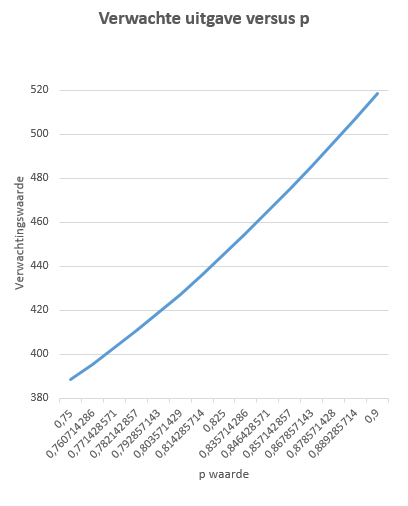
\includegraphics[scale=0.75]{HugoKR2}

In deze afbeelding kun je zien dat je al snel meer dan \euro450 per week kwijt bent, uitgaande van de startwaarde $p_{1} =0.75 + \frac{0.15}{14}$. Verder zien we dat de verwachte uitgave per week steeds harder gaat stijgen, terwijl p met een constante waarde stijgt. Dit is te verklaren door het feit dat er steeds meer loten optimaal benut zullen worden en dus steeds vaker de grootst mogelijke prijs van het lot gewonnen wordt. Dit heeft als gevolg dat in de loop van de krasactie, uitgaande van een lineaire p-stijging, er steeds meer uitgegeven zal moeten worden per week.\\

Wederom gebruikmakende van de waarden voor $\alpha$ t/m $d$, verkregen in de verdelingsanalyse, vinden we dat de verwachte totaaluitgaven in deze situatie gelijk zijn aan \euro12.340. Deze waarde ligt heel dichtbij het voorgeschreven budget van \euro12.300. Dit betekent dat de door ons bepaalde waarden van $\alpha, \beta, \gamma, \delta, a,b,c$ en $d$ ook geldig zijn voor de situatie dat alle postbezorgers steeds enthousiaster worden en dus $p$ lineair zal toenemen. De reden waarom dit werkt is omdat wij de waarden voor $\alpha$ t/m $d$ bepaald hebben bij een  standaardsituatie van $p = 0.83$ en dit ligt net boven het gemiddelde van $0.75$ en $0.9$. De sterkere stijging in de verwachte uitgave op het einde kan hierdoor worden ``geneutraliseerd'' en de verwachte waarde voor de totaaluitgaven zal daarom rond het budget van \euro12.300 blijven.  


\section{Nauwkeurigheidsmarge}

In de vorige paragraaf hebben we de parameters $\alpha, \beta, \gamma, \delta, a,b,c$ en $d$ vastgesteld. Nu willen we graag bekijken hoeveel zekerheid we het Eindhovens Dagblad kunnen bieden, uitgaande van deze parameters. We doen dit door gebruik te maken van de Centrale limietstelling, waarbij $p$ constant blijft gedurende de gehele periode waarin de krasactie loopt.\\

We zijn benieuwd naar de kans dat, gebruikmakende van ons model en onze parameters, de totale uitgaven binnen een bepaalde marge van het voorgeschreven budget (\euro12.300) uit zullen vallen. Wij kiezen eerst een marge van 5$\% \,(=615)$. Dat wil zeggen dat we gaan onderzoeken hoe groot de kans is dat de totale uitgaven binnen het gebied \euro$12.300 \pm 615$ zullen uitvallen.\\

In de paramateranalyse hebben we voor de gekozen waarden van $\alpha$ t/m $d$ de verwachtingswaarde en variantie bepaald van de uitgaven over exact één week. We bekijken nu de som $Z_{1} + \ldots + Z_{14}$, die de totaaluitgaven weergeven (over 14 weken). We moet hier wel de opmerking maken dat dit niet geheel juist is omdat we nu het gegarandeerde bedrag van \euro6000 vergeten mee te nemen, zoals in vergelijking (3.9) wel gebeurt. Dit probleem is echter makkelijk op te lossen door dit bedrag van het voorgeschreven budget af te trekken, ofwel:

\begin{equation*}
\sum_{i=1}^{14} \left( \mathbb{E}[Z_{i}] \right) + 6000 = 12.300
\end{equation*}
geeft
\begin{equation*}
\sum_{i=1}^{14} \left( \mathbb{E}[Z_{i}] \right) = 6.300.
\end{equation*}

Het bereik van de uitgaven dat we nu onderzoeken, ligt zodoende tussen de (\euro6300 $-$ \euro615 =) \euro5685 en (\euro6300 $+$ \euro615 =) \euro6915 . We passen nu de centrale limietstelling toe.\\

Allereerst merken we op dat we de centrale limietstelling hier mogen toepassen, omdat we te maken hebben met een som van 14 iid random variabelen. We hebben de aanname gemaakt dat de uitgaven per week onafahankelijk zijn van elkaar en omdat we de loten elke week met dezelfde verdeling verspreiden zijn deze gelijk verdeeld. Dit is ook de reden waarom we hier $p$ constant houden. Uiteraard is het verder natuurlijk zo dat er sprake is van een eindige variantie.\\

Er geldt dat $\mathbb{E}[Z_{i}] = \mu \approx 450$ en $Var(Z_{i}) = \sigma^{2}\approx 15.973$, zoals we hebben gezien in de parameteranalyse. We standaardiseren nu de som $Z_{1} + \ldots + Z_{14}$, waarbij we ge\"interesseerd zijn in $\mathbb{P}(5685 \leq Z_{1} + \ldots + Z_{14} \leq 6915)$. Deze herschrijven we als volgt:

%\begin{equation*}
\begin{eqnarray*}
\begin{aligned}
\lefteqn{\mathbb{P}\left(5685 \leq Z_{1} + \ldots + Z_{14} \leq 6915  \right)}\\ 
& \qquad{}= \mathbb{P}\left(\frac{5685 - 14 \cdot 450}{\sqrt{14 \cdot 15.973}} \leq \frac{Z_{1} + \ldots + Z_{14} - 14\mu }{\sqrt{14\sigma^{2}}} \leq \frac{6915 - 14 \cdot 450}{\sqrt{14 \cdot 15.973}}\right)\\
& \qquad{}\approx \mathbb{P}\left(-1.301 \leq Z \leq 1.301 \right)\\
&\qquad{}= \mathbb{P}(Z \leq 1.301) - \mathbb{P}(Z \leq -1.301)\\
&\qquad{}= \Phi(1.301)-\Phi(-1.301)\\
&\qquad{}= 2\Phi(1.301)-1\\
&\qquad{}\approx 2 \cdot 0.9032 - 1 \\
& \qquad{} \approx 0.81
\end{aligned}
\end{eqnarray*}
%\end{equation*}

We vinden dus dat de kans dat de totaaluitgaven binnen een marge van 5$\%$ rond het voorgeschreven budget uit zullen vallen ruwweg 4 op 5 is. Hoewel deze kans sterk ``in ons voordeel'' is, zijn wij echter van mening dat een kans van 1 op 5 dat dit niet het geval is iets te groot om de opdrachtgever mee gerust te kunnen stellen. Daarom besluiten we de berekening te herhalen voor een iets grotere marge, namelijk 7,5$\%$, wat neerkomt op \euro922,50. Het nieuwe bereik voor de totaaluitgaven loopt dan van \euro5377,50 tot \euro7222,50. Op dezelfde manier als hierboven herschrijven we nu $\mathbb{P}(5377,50 \leq Z_{1} + \ldots + Z_{14} \leq 7222,50)$:

\begin{eqnarray*}
\begin{aligned}
\lefteqn{\mathbb{P}\left(5377,50 \leq Z_{1} + \ldots + Z_{14} \leq 7222,50  \right)}\\ 
& \qquad{}= \mathbb{P}\left(\frac{5377,50 - 14 \cdot 450}{\sqrt{14 \cdot 15.973}} \leq \frac{Z_{1} + \ldots + Z_{14} - 14\mu }{\sqrt{14\sigma^{2}}} \leq \frac{7222,50 - 14 \cdot 450}{\sqrt{14 \cdot 15.973}}\right)\\
& \qquad{}\approx \mathbb{P}\left(-1.951 \leq Z \leq 1.951 \right)\\
&\qquad{}= 2\Phi(1.951)-1\\
&\qquad{}\approx 2 \cdot 0.9744 - 1 \\
& \qquad{} \approx 0.95
\end{aligned}
\end{eqnarray*}

Nu vinden we een veel gerustellendere kans van 19 op 20 dat de totaaluitgaven binnen een marge van 7,5$\%$ rond het voorgeschreven budget zullen uitvallen. Dit is naar onze mening een acceptabele nauwkeurigheidsmarge die we de opdrachtgever mogen meegeven.